\documentclass[10pt,letterpaper]{article}
\usepackage[utf8]{inputenc}
\usepackage{amsmath}
\usepackage{amsfonts}
\usepackage{amssymb}
\usepackage{graphicx}
\usepackage{siunitx}
\DeclareSIUnit{\torr}{torr}
\sisetup{retain-unity-mantissa = false}
\usepackage{booktabs}
\usepackage{ulem}

\author{W. Schreyer, S. Morawetz}
\title{Fall run 2018 -- analysis report}
\begin{document}

\maketitle

\tableofcontents

\section{Introduction}

This document describes several analyses of the data taken during the 2018 run of the UCN source at TRIUMF, covering measurements of
\begin{itemize}
\item transmission through guide components
\item storage lifetime in the source, and
\item storage lifetime in guide components.
\end{itemize}

All these experiments are performed in cycles. Each cycle contains several periods, typically starting with an irradiation period, during which the target is irradiated with protons and ultracold neutrons are produced. This can be followed by up to 9 more periods, like storage or detection periods. For each period, up to 8 UCN components like valves or spin flippers can be to set different states. The last (11th) period covers the time until the next irradiation and cycle starts.

Cycles with different period durations and valve settings can be grouped in supercycles, which can be repeated several times. Cycles of one experiment can be spread over several Midas runs.

Two UCN detectors were used throughout the run. A Li6 detector, detecting scintillation light of UCN captured in $^6$Li-enriched glass, and a He3 detector, detecting gas discharges due to UCN captured by $^3$He. Experiments can use either detector alone or both at the same time.


\section{Preparation of raw detector data}

\subsection{Trigger thresholds}

The Li6 detector uses two values to determine if a detected event was actually caused by a UCN: ``PSD'' based on the pulse shape of the event and $Q_\mathrm{long}$, the charge collected during a \SI{200}{\nano\second} window after the event trigger. An event is considered a UCN if
\begin{equation}
\mathrm{PSD} > 0.3
\end{equation}
and
\begin{equation}
Q_\mathrm{long} > 2000.
\end{equation}

The He3 detector considers an event to be a UCN if the charge collected after the event trigger
\begin{equation}
Q_\mathrm{short} > 300.
\end{equation}

\subsection{Excluded events}

In some experiments with high gas pressures in the UCN guide we saw the rate in the Li6 detector spike when a valve moved. Affected runs identified so far are 1153 to 1160 and 1203 to 1205. These were all part of measurements at high He-II temperatures and high vapor pressures, or measurements with high nitrogen pressures injected into the UCN guide. In these runs, the events in the Li6 detector within the first second of each period were binned into \SI{1}{\milli\second}-wide bins and all events in bins that had more than three entries were discarded. In total, about \num{70000} events were discarded from 72 cycles this way.


\section{Transmission measurements}

Transmission measurements are experiments with two periods per cycle. An irradiation period, $t_i$, where UCN are produced and a small percentage is detected in the He3 detector connected to a monitoring port while a valve downstream of the He3 detector is closed. And a counting period, $t_c$, where the UCN valve is opened and UCN transmitted through components downstream of the valve are detected in the Li6 detector.

\subsection{Normalization during counting}

When the valve is opened, UCN start to reach the Li6 detector. But a small part can be absorbed on the guides between the valve and the Li6 detector, or scattered back towards the He3 detector and source, reducing the number of UCN seen in the Li6 detector and increasing the number of UCN seen in the He3 detector during the counting period. Hence, the ratio
\begin{equation}
R_c = \frac{N^\mathrm{Li6}_c}{N^\mathrm{He3}_c}
\end{equation}
of UCN seen in the Li6 detector $N^\mathrm{Li6}_c$ to the UCN seen in the He3 detector $N^\mathrm{He3}_c$ is a measure of how well UCN can be transmitted through the guides between the valve and the Li6 detector.

A constant background rate $b^\mathrm{Li6}$ (see section \ref{sec:background}) is subtracted from the number of events counted in the Li6 detector during counting $C^\mathrm{Li6}_c$:
\begin{equation}
\label{eq:transmission_begin}
N^\mathrm{Li6}_c = C^\mathrm{Li6}_c - b^\mathrm{Li6} \cdot t_c,
\end{equation}
with an uncertainty
\begin{equation}
\Delta N^\mathrm{Li6}_c = \sqrt{ \sqrt{C^\mathrm{Li6}_c}^2 + \left( \Delta b^\mathrm{Li6} \cdot t_c \right)^2}.
\end{equation}

The uncertainty of the ratio $R$ is then
\begin{equation}
\Delta R_c = \sqrt{ \left( \frac{\Delta N^\mathrm{Li6}_c}{N^\mathrm{He3}_c} \right)^2 + \left( \sqrt{N^\mathrm{He3}_c} \frac{N^\mathrm{Li6}_c}{{N^\mathrm{He3}_c}^2} \right)^2  }.
\end{equation}
The He3 detector is assumed to be background-free.

\begin{figure}
\centering
\includegraphics[width=\textwidth,page=1]{{"../transmission/TCN18-045 (IV2+UGD22+IV3, O-rings in)"}.pdf}
\includegraphics[width=\textwidth,page=2]{{"../transmission/TCN18-045 (IV2+UGD22+IV3, O-rings in)"}.pdf}
\caption{Ratio of Li6 counts to He3 counts during the counting period (top) and during the last \SI{10}{\second} of the irradiation period (bottom). All cycles of transmission experiment TCN18-045 are shown and fitted with a constant function. The legend shows the $\chi^2/\nu$ of the fit, the average ratio $\bar{R}$, and its uncertainty.}
\label{fig:transmission}
\end{figure}

The ratios for all cycles are plotted using ROOT. A $\chi^2$ fit of a constant function over all cycles is used to determine the average $\bar{R}_c$ and its uncertainty $\Delta \bar{R}_c$, see figure~\ref{fig:transmission}. Table~\ref{tab:transmission} shows the results for all performed transmission experiments.

The relative transmission $T$ of one experiment compared to another is
\begin{equation}
T_c = \frac{\bar{R}_{c1}}{\bar{R}_{c2}}
\end{equation}
with the uncertainties for each $\bar{R}_c$ scaled by the $\chi^2$ per degrees of freedom $\nu$ from the fit:
\begin{equation}
\label{eq:transmission_end}
\Delta T_c = T_c \sqrt{ \left( \frac{\Delta \bar{R}_{c1} \chi_1^2}{\bar{R}_{c1} \nu_1} \right)^2 + \left( \frac{\Delta \bar{R}_{c2} \chi_2^2}{\bar{R}_{c2} \nu_2} \right)^2 }.
\end{equation}
Comparisons of transmission through different guide geometries are shown in table~\ref{tab:transmission_comparison}.


\subsection{Normalization during irradiation}

Another measure of transmission would be the the number of UCN that make it to the Li6 detector $N^\mathrm{Li6}_c$ divided by the number of UCN that are available in the source at the moment the valve opens $N_\mathrm{src}(t_i)$.
If we assume that the rate in the monitor detector $r_\mathrm{He3}(t)$ is proportional to the number of UCN in the source, this transmission would be given by

\begin{equation}
R = \frac{N_c^\mathrm{Li6}}{r_\mathrm{He3}(t_i)} \propto \frac{N_c^\mathrm{Li6}}{N_\mathrm{src}(t_i)} .
\end{equation}

The rate in the monitor detector is small and to determine the rate right when the valve opens requires an integration over a time window $\Delta t$ wide enough to reduce statistical uncertainties to an acceptable level:
\begin{equation}
r_\mathrm{He3}(t_i) \approx \frac{1}{\Delta t} \int_{t_i - \Delta t}^{t_i}  r_\mathrm{He3}(t)
\end{equation}
However, the wider the time window the more the measurement of the instantaneous rate is affected by changes in the storage lifetime in the source. E.g. if we assume a simple model for the number of UCN in the source
\begin{equation}
r_\mathrm{He3}(t) \propto N_\mathrm{src}(t) = N_0 \left( 1 - e^{-t/\tau} \right)
\end{equation}
the proportionality constant
\begin{equation}
\epsilon_\mathrm{He3} = \frac{r_\mathrm{He3}(t_i)}{N_\mathrm{src}(t_i)} = \frac{\int_{t_i - \Delta t}^{t_i} 1 - e^{-t/\tau}}{1 - e^{-t_i/\tau}}
\end{equation}
is more affected by a change in the storage lifetime $\tau$ if the time windows $\Delta t$ is wider. If the time window spanned the full \SI{60}{\second} irradiation time, a change in storage lifetime from \SIrange{37}{27}{\second} (see section \ref{sec:storagelifetime}) would result in a \SI{7}{\percent} change in the proportionality constant; if the time window is only \SI{10}{\second} wide the resulting change would only be \SI{1}{\percent}.

A change in storage lifetime would similarly affect the number of UCN in the Li6 detector. The shorter the storage lifetime in the source, the less UCN would make it to the Li6 detector, even if the initial number of UCN and the guide geometry is the same. If we use a simple model of the rate in the Li6 detector
\begin{equation}
r_\mathrm{Li6}(t) = N_0 e^{-t/\tau_2}
\end{equation}
we can compare the rates integrated over the counting time
\begin{equation}
N^\mathrm{Li6}_c = \int_{t_i}^{t_i+t_c} r_\mathrm{Li6}(t)
\end{equation}
between experiments where $\tau_2$ changes from \SIrange{12}{13}{\second}. If the counting time is \SI{60}{\second}, this would result in a change of the detected number of \SI{7}{\percent}, if the counting time is \SI{10}{\second}, the change is reduced to \SI{3}{\percent}.

These effects on the He3 and Li6 rates compound each other and can lead to considerable systematic differences between identical transmission experiments with varying source lifetime.

Additionally, a major change of the transmission geometry would also affect the time constant $\tau_2$, making it impossible to compare experiments with significantly different guide lengths or volumes. Fortunately, for every transmission experiment, we performed reference measurements with similar guide length that we can compare to even with this analysis method.

The normalization during counting should be much less affected by changes in these time constants, since the rates in the He3 and Li6 detectors are measured at the same time and are subject to the same time constant $\tau_2$. This implies the assumption that the time needed to bring the rates in both detectors to an equilibrium is much shorter than $\tau_2$.

To minimize systematic uncertainties of the normalization during irradiation, we integrated the He3 and Li6 rates over \SI{10}{\second}-long time windows. The beginning of the Li6 time window was set to the time when the rate suddenly increases to compensate any jitter in valve actuation. Background subtraction and uncertainty estimation were performed similarly to equations (\ref{eq:transmission_begin})--(\ref{eq:transmission_end}), leading to ratios $\bar{R}_i$ and $T_i$ and their corresponding uncertainties, see table \ref{tab:transmission}.

\subsection{Excluded cycles}

Individual cycles are excluded from the analyzed transmission data if
\begin{itemize}
\item the beam current dropped below \SI{0.1}{\micro\ampere} (10 cycles);
\item the beam current fluctuated by more than \SI{0.02}{\micro\ampere} (10 cycles);
\item the last period does not contain any Li6 events, i.e. the run was aborted at some point during this cycle (35 cycles);
\item IV1 never opened (3 cycles);
\item the ion gauge IG6 read a pressure between \SIlist{1e-7;1e-2}{\torr}, indicating that it was on, causing additional background in the Li6 detector (88 cycles);
\item the Li6 detector detected an average rate below \SI{10}{\hertz} during the counting period (0 cycles); or
\item the Li6 detector detected a large background rate above \SI{10}{\hertz} during the irradiation period (4 cycles).
\item the He3 detector detected less than 300 UCN during counting (3 cycles);
\end{itemize}

In total, 153 out of 579 cycles were excluded. All cycles of experiments TCN18-028 (run 929)  TCN18-029 (run 934) and TCN18-080 (run 973) had to be discarded, due to IG6 being on.

\subsection{Results}

\begin{table}
\centering
\caption{Results of transmission experiments. If not otherwise noted, all transmission measurements were performed with the listed guides between IV2 and IV3 with their O-rings pointing towards each other and a 90$^\circ$ elbow downstream of IV3. The $\chi^2$ gives an indication of how well the data fits the assumption that the ratios $R$ stay constant over all cycles in each experiment.}
\makebox[\textwidth]{
\begin{tabular}{l r r r r r p{0.4\textwidth}}
\toprule
Experiment & Run & $\bar{R}_c$ & $\chi^2/\nu$ & $\bar{R}_i$ & $\chi^2/\nu$ & Description \\
\midrule
TCN18-031 & 938 & $34.92 \pm 0.27$ & 1.01 & $25.31 \pm 0.24$ & 1.02 & UGD17, no IV3 \\
TCN18-035 & 944 & $31.26 \pm 0.26$ & 0.68 & $22.92 \pm 0.23$ & 1.48 & UGD22, O-rings of IVs pointing away from each other \\
TCN18-045 & 954 & $31.78 \pm 0.27$ & 2.45 & $23.87 \pm 0.25$ & 0.97 & UGD22 \\
TCN18-053 & 985 & $32.71 \pm 0.29$ & 2.19 & $22.81 \pm 0.24$ & 0.47 & burst disk + UGD2 \\
TCN18-085 & 973 & $32.78 \pm 0.30$ & 1.38 & $23.23 \pm 0.25$ & 0.77 & UGD22 + 19 (NiP) \\
TCN18-090 & 1000 & $29.21 \pm 0.27$ & 1.47 & $21.61 \pm 0.24$ & 1.39 & UGD22 + UGA11 + UGG3 + UGA5 \\
TCN18-290 & 1009 & $30.36 \pm 0.29$ & 2.57 & $21.32 \pm 0.24$ & 0.56 & UGD22 + UGA5 + UGG3 + UGA6 \\
TCN18-060 & 1013 & $32.09 \pm 0.30$ & 0.61 & $22.80 \pm 0.25$ & 1.88 & UGD10 + 17 + 11 \\
TCN18-065 & 1054 & $31.06 \pm 0.26$ & 1.63 & $21.33 \pm 0.21$ & 0.59 & SCM warm bore \\
TCN18-265 & 1081 & $15.43 \pm 0.14$ & 0.78 & $12.09 \pm 0.14$ & 1.12 & SCM warm bore with foil \\
TCN18-115 & 1125 & $18.74 \pm 0.18$ & 1.51 & $14.00 \pm 0.16$ & 0.83 & UGD22 + 2 + Ti foil \\
TCN18-245 & 1129 & $32.42 \pm 0.28$ & 2.42 & $24.33 \pm 0.26$ & 2.00 & UGD22 (repeat) \\
TCN18-480 & 1131 & $32.84 \pm 0.30$ & 0.84 & $22.96 \pm 0.25$ & 0.33 & UGD22 + 2 \\
TCN18-057 & 1141 & $30.70 \pm 0.27$ & 1.69 & $22.11 \pm 0.24$ & 0.42 & vent spider + UGD2 \\
\midrule
\multicolumn{5}{l}{Experiments at high position:} \\
TCN18-302 & 1165 & $48.88 \pm 0.34$ & 3.89 & $31.81 \pm 0.25$ & 1.14 & IV2 + elbow + UGD10 + 18 \\
TCN18-240 & 1176 & $24.18 \pm 0.17$ & 3.80 & $18.53 \pm 0.17$ & 1.04 & IV2 + elbow + UGD10 + Al foil + UGD18 \\
TCN18-215 & 1181 & $18.55 \pm 0.15$ & 1.16 & $13.42 \pm 0.13$ & 1.21 & UGD22 + 20 + Ti foil \\
TCN18-380 & 1188 & $41.52 \pm 0.35$ & 1.93 & $28.94 \pm 0.30$ & 1.25 & UGD22 + 20 \\
TCN18-310 & 1192 & $50.84 \pm 0.35$ & 1.50 & $32.14 \pm 0.26$ & 0.97 & UGD22 + 20, smooth elbow \\
\bottomrule
\end{tabular}
}
\label{tab:transmission}
\end{table}

\begin{table}
\centering
\caption{Comparison of transmission experiments. The struck-out entries of $T_i$ are invalid comparisons of setups with different lengths and are included only for reference.}
\makebox[\textwidth]{
\begin{tabular}{l r r r p{0.4\textwidth}}
\toprule
Experiment & Reference & $T_c$ & $T_i$ & Description \\
\midrule
TCN18-045 & TCN18-245 & $0.980 \pm 0.029$ & $0.981 \pm 0.023$ & Comparison of reference measurements \\
TCN18-035 & TCN18-031 & $0.895 \pm 0.010$ & $0.906 \pm 0.016$ & UGD22+IV3 compared to UGD17\\
TCN18-045 & TCN18-035 & $1.017 \pm 0.023$ & $1.041 \pm 0.018$ & Flipping IV2 and IV3\\
TCN18-053 & TCN18-045 & $1.029 \pm 0.029$ & \sout{$0.955 \pm 0.015$} & Replacing UGD22 with burst disk and UGD2 \\
TCN18-053 & TCN18-480 & $0.996 \pm 0.022$ & $0.994 \pm 0.015$ & Burst disk compared to UGD22 \\
TCN18-057 & TCN18-053 & $0.939 \pm 0.023$ & $0.969 \pm 0.014$ & Vent spider compared to burst disk \\
TCN18-085 & TCN18-045 & $1.031 \pm 0.025$ & \sout{$0.973 \pm 0.015$} & Adding UGD19 (NiP) \\
TCN18-085 & TCN18-480 & $0.998 \pm 0.015$ & $1.012 \pm 0.015$ & UGD19 (NiP) compared to UGD2 \\
TCN18-090 & TCN18-045 & $0.919 \pm 0.023$ & \sout{$0.905 \pm 0.017$} & Adding UGG3 with UGA11+3 \\
TCN18-090 & TCN18-480 & $0.900 \pm 0.015$ & $0.941 \pm 0.017$ & UGG3 with UGA11+3 compared to UGD2 \\
TCN18-290 & TCN18-045 & $0.955 \pm 0.031$ & \sout{$0.893 \pm 0.015$} & Adding UGG3 with UGA5+6\\
TCN18-290 & TCN18-480 & $0.924 \pm 0.024$ & $0.929 \pm 0.015$ & UGG3 with UGA5+6 compared to UGD2\\
TCN18-060 & TCN18-045 & $1.010 \pm 0.023$ & \sout{$0.955 \pm 0.024$} & Replacing UGD22 with UGD10 + 17 + 11 \\
TCN18-065 & TCN18-045 & $0.977 \pm 0.024$ & \sout{$0.894 \pm 0.014$} & Replacing UGD22 with SCM warm bore \\
TCN18-065 & TCN18-060 & $0.968 \pm 0.016$ & $0.936 \pm 0.022$ & Warm bore compared to UGD10 + 17 + 11 \\
TCN18-265 & TCN18-065 & $0.497 \pm 0.008$ & $0.567 \pm 0.008$ & Adding foil to SCM warm bore \\
TCN18-115 & TCN18-480 & $0.571 \pm 0.010$ & $0.610 \pm 0.009$ & Adding Ti foil \\
TCN18-480 & TCN18-045 & $1.033 \pm 0.024$ & \sout{$0.962 \pm 0.016$} & Adding UGD2 \\
TCN18-057 & TCN18-045 & $0.966 \pm 0.025$ & \sout{$0.926 \pm 0.014$} & Replacing UGD22 with vent spider and UGD2 \\
\midrule
\multicolumn{4}{l}{Experiments at high position:} \\
TCN18-240 & TCN18-302 & $0.495 \pm 0.019$ & $0.582 \pm 0.007$ & Adding Al foil after \SI{50}{\centi\meter} drop \\
TCN18-215 & TCN18-380 & $0.447 \pm 0.008$ & $0.464 \pm 0.008$ & Adding Ti foil in horizontal guide \\
TCN18-310 & TCN18-380 & $1.224 \pm 0.024$ & $1.111 \pm 0.019$ & Smooth compared to mitered elbow\\
\bottomrule
\end{tabular}
}
\label{tab:transmission_comparison}
\end{table}

Table \ref{tab:transmission} lists the results of the individual transmission experiments and table \ref{tab:transmission_comparison} compares several.

Most measurements give compatible results with both normalization methods, but the normalization during irradiation generally gives smaller $\chi^2/nu$ values.
\begin{itemize}
\item The two identical reference measurements TCN18-045 and -245 show no significant difference in transmissions.
\item The VAT valves have a transmission of \SI{90}{\percent}.
\item Flipping the VAT valves might have increased transmission slightly by about \SI{3}{\percent}.
\item A bare stainless-steel guide had similar transmission as a stainless-steel guide plated with NiP.
\item The NiMo-coated glass guide with flange adapters had only \SI{92}{\percent} of the transmission of the bare and coated stainless-steel guides.
\item The burst-disk holder did not significantly reduce transmission compared to a bare stainless-steel guide with same length.
\item The ``vent spider'' reduced transmission to \SI{95}{\percent} compared to the burst-disk holder or a stainless-steel guide of same length.
\end{itemize}
The largest discrepancies between the two normalization methods are seen in measurements that have a large effect on the number of UCN reflected back towards the source and He3 detector, e.g. adding a foil or replacing the elbow leading down to the Li6 detector:
\begin{itemize}
\item Adding a \SI{100}{\micro\meter}-thick aluminium foil into the SCM warm bore reduced transmission to \SIlist{50;57}{\percent}.
\item Adding a \SI{100}{\micro\meter}-thick aluminium foil into a \SI{1}{\meter}-high drop into the Li6 detector reduced transmission to \SIlist{50;58}{\percent}.
\item Adding a \SI{15}{\micro\meter}-thick titanium foil reduced transmission to \SIlist{57;61}{\percent} (at the lower position, higher UCN energies) or to \SIlist{45;46}{\percent} (at the higher position, lower UCN energies).
\item Replacing the mitered elbow with a bare, smooth elbow increased transmission by \SIlist{22;11}{\percent}.
\end{itemize}

Interestingly, some setups that have a \SI{1}{\meter}-long guide inserted (TCN18-085, -480) seem to have larger transmissions $T_c$ than the setup without the guide (TCN18-045); most likely because the added guide reduces back-scatter from the elbow attached at the end of each setup.

\subsection{Time dependence of detector rates}

\begin{figure}
\centering
\includegraphics[width=\textwidth,page=4]{{"../transmission/TCN18-045 (IV2+UGD22+IV3, O-rings in)"}.pdf}
\caption{Rate in the He3 detector during transmission experiment TCN18-045, summed over all cycles.}
\label{fig:he3rate}
\end{figure}

The rate in the He3 detector initially increases and would eventually saturate when the UCN-production rate equals the loss rate in the source, and then drops off exponentially after the valve is opened. A simple model to describe the probability of a UCN diffusing from the source at $x = 0$ into the He3 detector at $x = L$ is the solution of the diffusion equation multiplied with an exponential decay describing the loss over time\footnote{A more accurate model would be the full solution to the non-stationary diffusion equation $\partial_t n = \partial_{xx} n - n$, which has no analytical solution}:
\begin{equation}
n(L, t) = \sqrt{\frac{\tau_d}{L^2 \pi t}} \exp \left( -\frac{\tau_d}{t} \right) \exp \left( -\frac{t}{\tau} \right),
\end{equation}
where $\tau_d$ is the average time the UCN need to diffuse from the source to the detector and $\tau$ is the storage lifetime in the source. Convolving this model with a constant production rate from $t = 0$ to $t_i$ gives the rate during the irradiation time
\begin{equation}
r_\mathrm{He3}(t) = p_0
\left[
  \mathrm{erfc} \left(
    \sqrt{\frac{\tau_d}{t}} - \sqrt{\frac{t}{\tau}}
  \right)
  - \exp \left(
    4 \sqrt{\frac{\tau_d}{\tau}}
  \right)
  \mathrm{erfc} \left(
    \sqrt{\frac{\tau_d}{t}} + \sqrt{\frac{t}{\tau}}
  \right) 
\right],
\end{equation}
where erfc is the complementary error function. Fitting this function to the measured rate gives diffusion time constants in the range \SIrange{10}{14}{\second} and storage lifetimes from \SIrange{30}{40}{\second}, see fig.~\ref{fig:he3rate}, similar to the actually measured storage lifetimes, see section~\ref{sec:storagelifetime}. The uncertainties are large, however.

\begin{figure}
\centering
\includegraphics[width=\textwidth,page=5]{{"../transmission/TCN18-045 (IV2+UGD22+IV3, O-rings in)"}.pdf}
\caption{Rate in the Li6 detector during transmission experiment TCN18-045, summed over all cycles.}
\label{fig:li6rate}
\end{figure}

The rate in the Li6 detector peaks very quickly after opening the valve, due to the usually short distance between valve and detector and then drops off exponentially. A model with a quick exponential saturation with time constant $\tau_\mathrm{rise}$, starting a short delay $t_d$ after the valve has opened, multiplied with the sum of three exponential decays turned out to fit the rate quite well, see fig.~\ref{fig:li6rate}:
\begin{equation}
r_\mathrm{Li6}(t > t_i + t_d) = p_0 \left( 1 - e^{-\frac{t}{\tau_\mathrm{rise}}} \right) \left(
e^{ -\frac{t}{\tau_1} } + 
N_2 e^{-\frac{t}{\tau_2}} + 
N_3 e^{ -\frac{t}{\tau_3} }
\right).
\end{equation}
Due to timing jitter in the valve actuation and different flight lengths between valve and detector, the delay $t_d$ can reach from \SIrange{1}{2}{\second}. Between cycles in one run, the delay varies by less than \SI{0.1}{\second}. The initial rise and fall times $\tau_\mathrm{rise}$ and $\tau_1$ are typically less than \SI{1}{\second}. The bulk of UCN has a storage lifetime $\tau_2$ of \SIrange{12}{15}{\second}. A smaller fraction, $N_3/N_2 \approx 0.1$, has a long storage lifetime $\tau_3$ of \SI{30}{\second} or more.

\begin{figure}
\centering
\includegraphics[width=\textwidth,page=8]{{"../transmission/TCN18-045 (IV2+UGD22+IV3, O-rings in)"}.pdf}
\caption{Ratio of rates in the Li6 detector and in the He3 detector during transmission experiment TCN18-045.}
\label{fig:rateratio}
\end{figure}

The ratio of the Li6 rate to the He3 rate quickly finds and equilibrium within about \SI{2}{\second} and is constant for the first \SI{60}{\second}, after which the statistical fluctuations quickly increase, see fig.~\ref{fig:rateratio}. This confirms that the assumptions necessary for the normalization method during counting are reasonable.

\begin{figure}
\centering
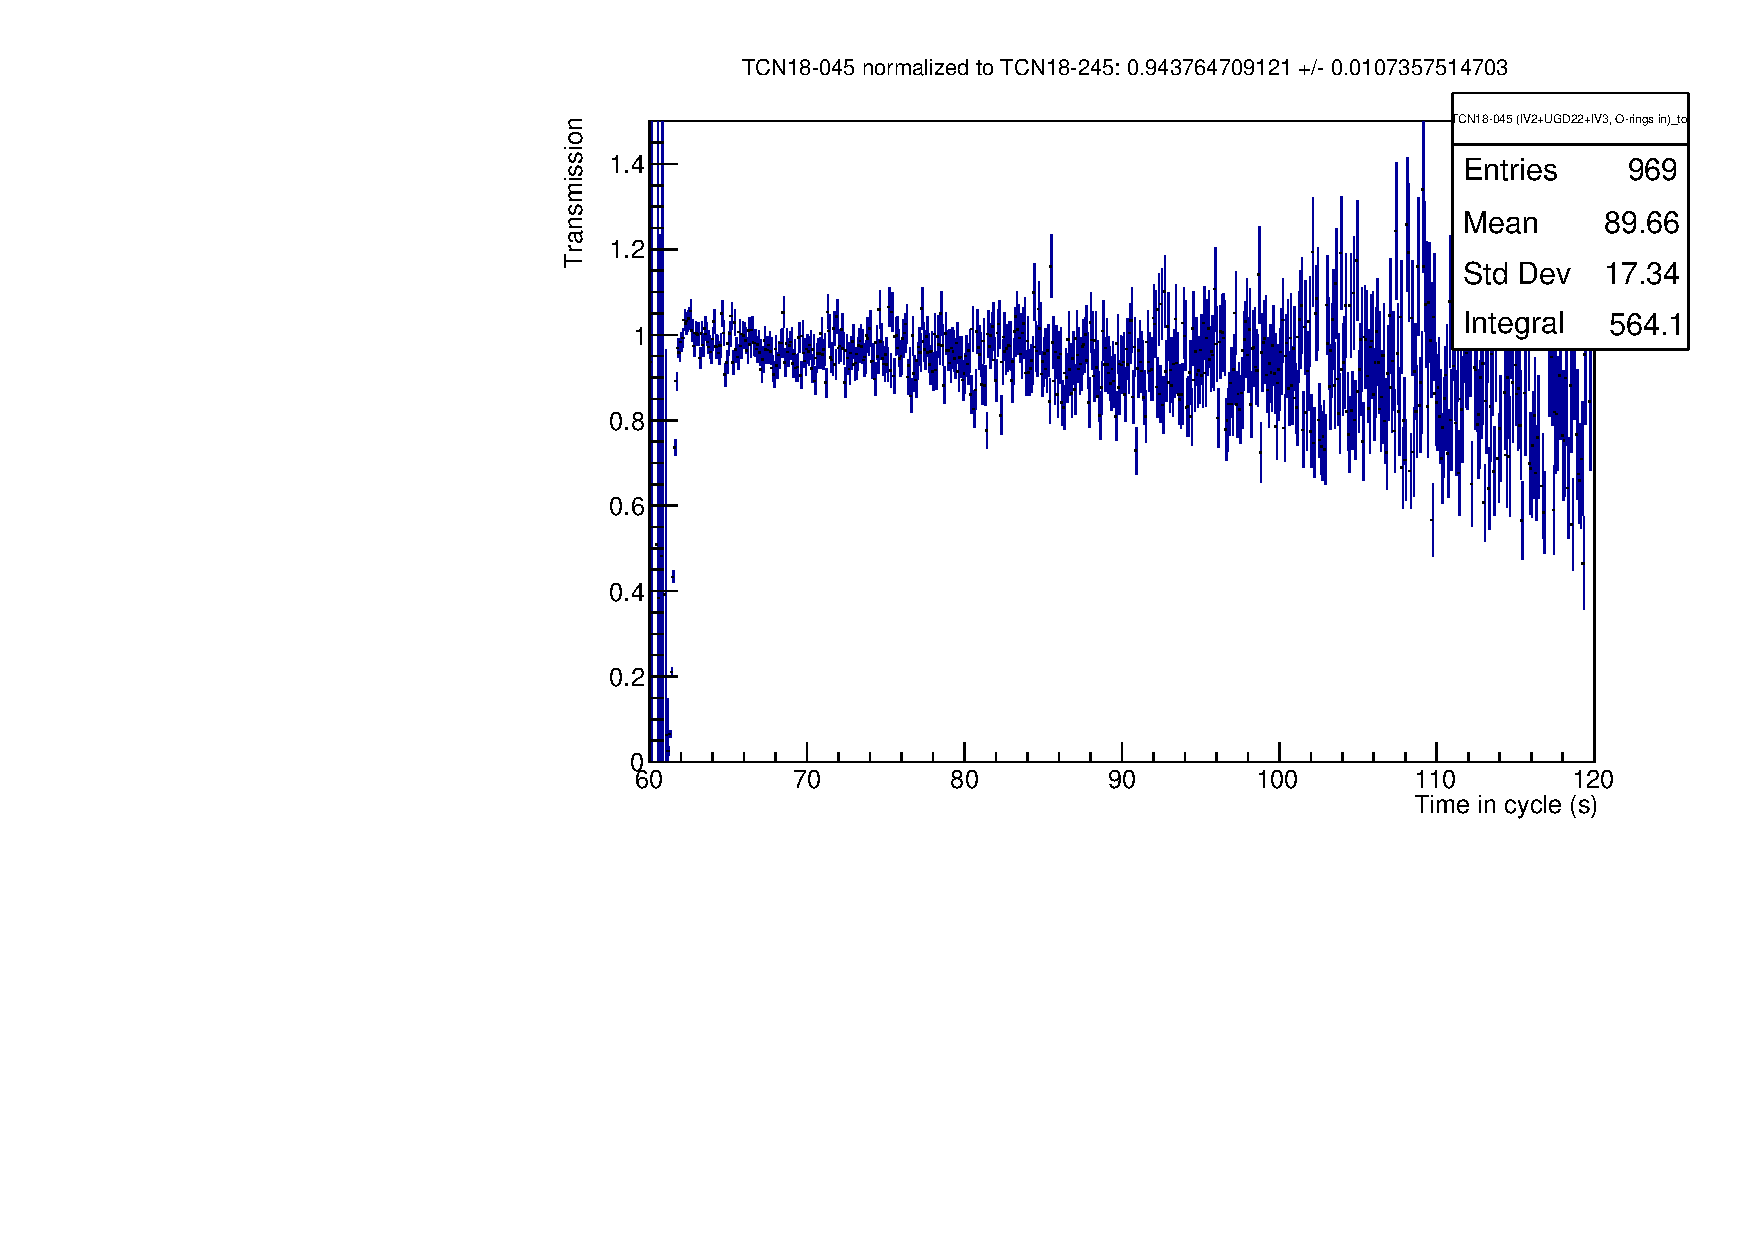
\includegraphics[width=\textwidth,page=1]{../transmission/TCN18-045_TCN18-245.pdf}
\caption{Ratio of normalized Li6-detector rates in identical experiments TCN18-045 and TCN18-245. The title contains the total relative transmission $T_c$. A slight decrease over time can be observed, likely due to a variation in storage lifetime in the source. The fast fluctuations in the beginning stem from jitter in the timing of the valve opening.}
\label{fig:rate_ratio_normalized}
\end{figure}

We can also normalize the background-corrected rate in the Li6 detector by dividing it by the normalization counts from the respective normalization methods. Averaging the normalized rate over all cycles and dividing it by the average normalized rate of a different experiment shows how the relative transmission changes over time, see figure~\ref{fig:rate_ratio_normalized}.

\subsection{SCM transmission}

We equipped the superconducting polarizer magnet (SCM) with a ``warm'' bore with an inner diameter of \SI{85}{\milli\meter} and an \SI{0.1}{\milli\meter}-thick AlMg3 foil in the center. Due to the tight fit of the guide through the cold superconducting magnet coil the foil could only be clamped between two narrow surfaces and was stripped out when we accidentally produced a pressure difference across the foil while pumping the guide. Hence, we did the first transmission measurements without a foil. We were able to insert a new foil soldered onto a thin stainless-steel ring later on and performed the same measurements with the foil inserted.

As seen in table~\ref{tab:transmission_comparison}, adding the warm bore without the foil (TCN18-065) reduced transmission to the Li6 detector by about \SI{5}{\percent} compared to stainless-steel guides with the same total length (TCN18-060), likely due to small gaps in the Wilson-style flanges holding the bore.

\begin{figure}
\centering
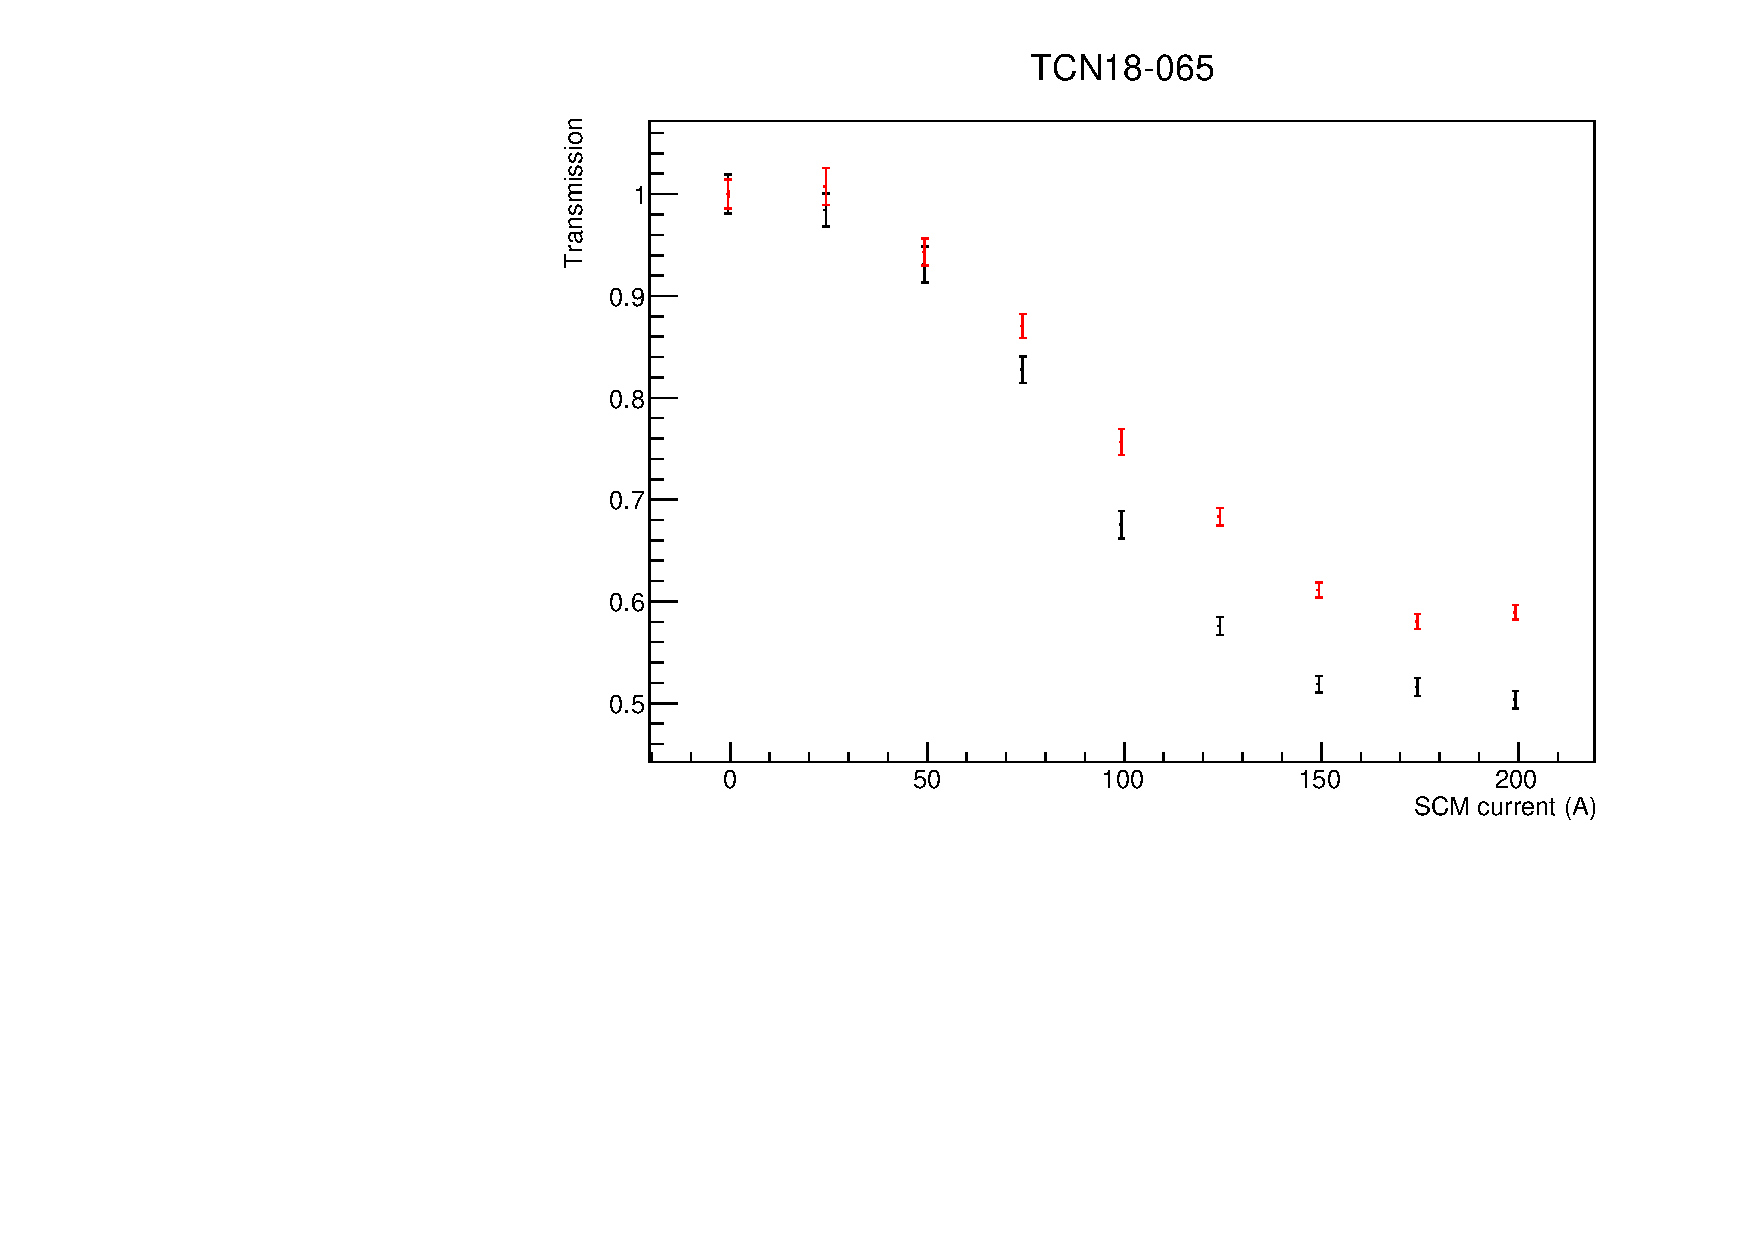
\includegraphics[width=\textwidth,page=1]{../transmission/TCN18-065.pdf}
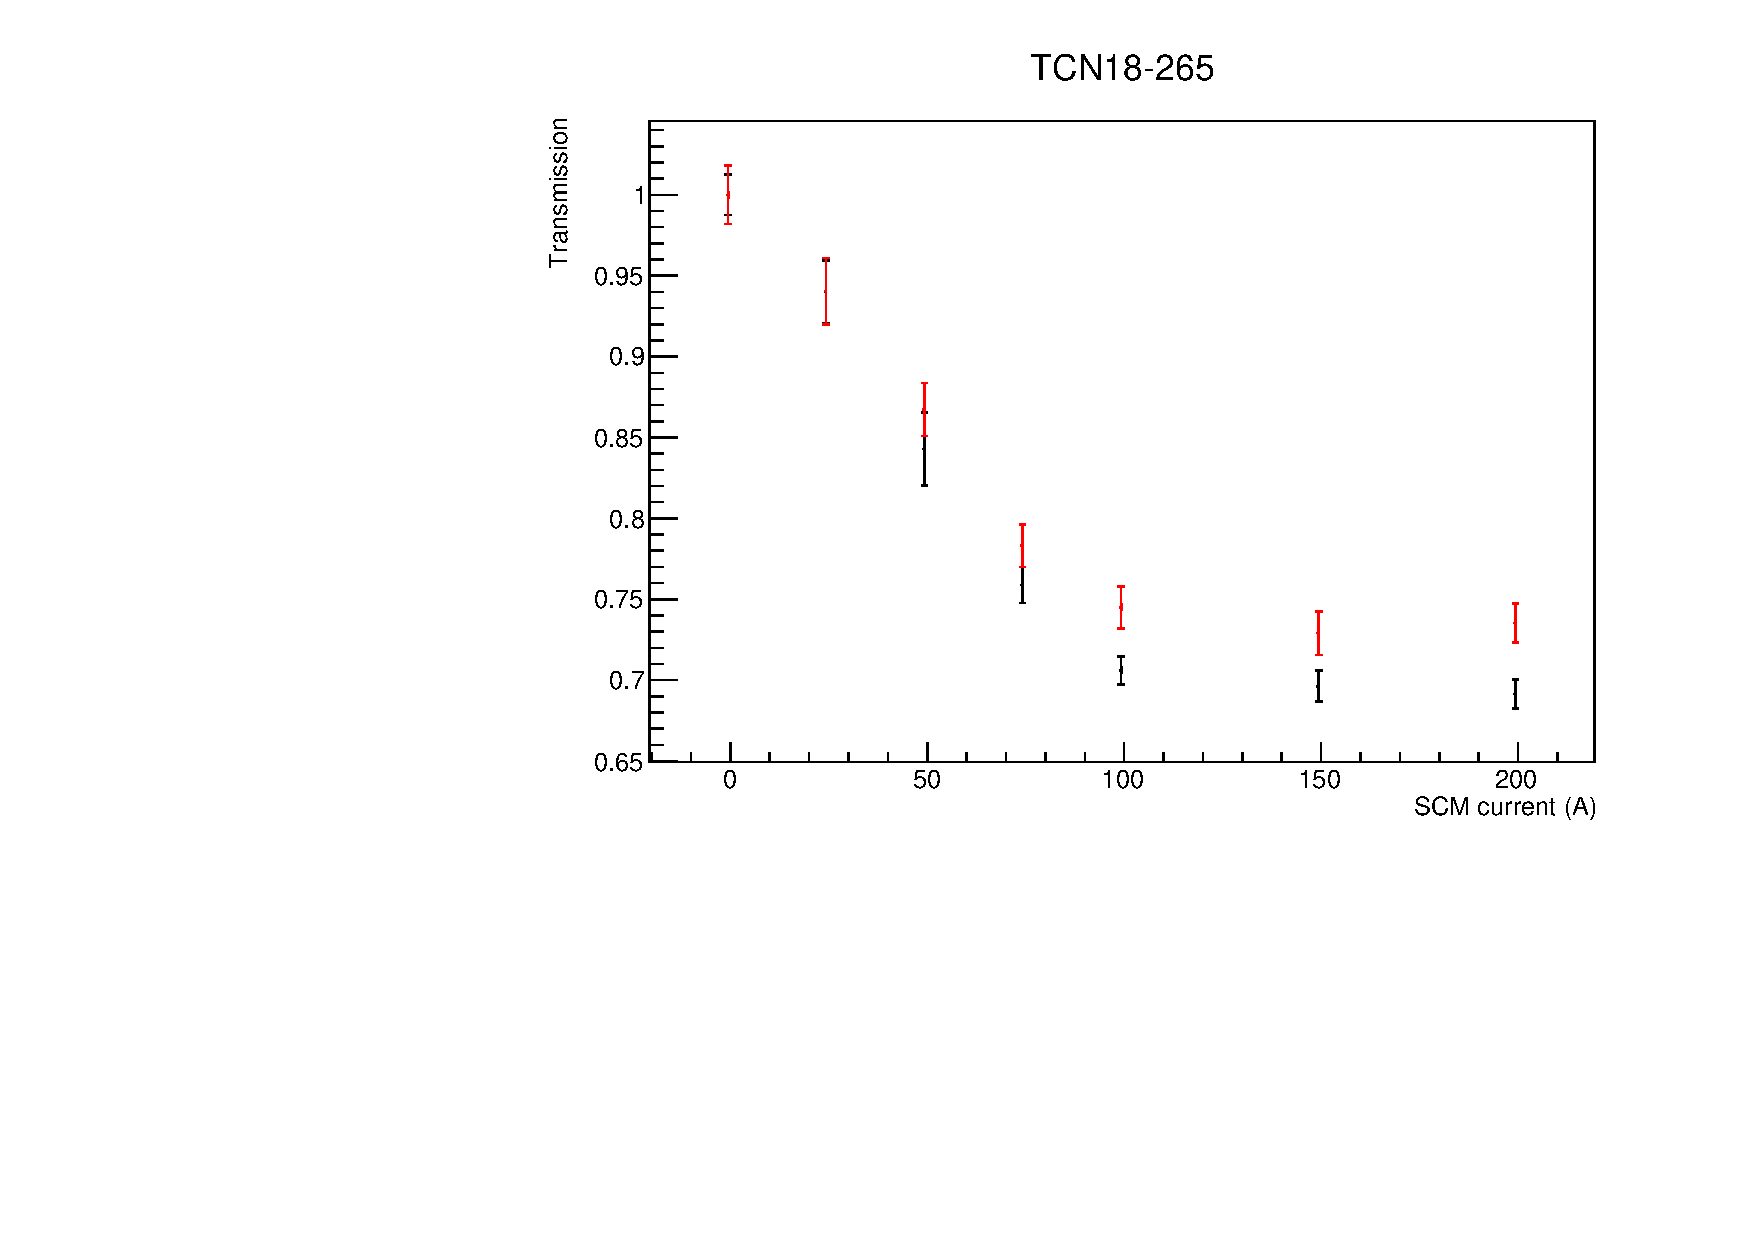
\includegraphics[width=\textwidth,page=1]{../transmission/TCN18-265.pdf}
\caption{Transmission $T$ through the warm bore while the SCM is powered with different currents, compared to transmission while unpowered. The black data points are calculated with the normalization during counting, the red data points with the normalization during irradiation. \textit{Top}: without foil; \textit{bottom}: with foil inserted.}
\label{fig:SCMtransmission}
\end{figure}

When the current in the SCM magnet is increased the magnetic field $B$ acts as a potential wall or trough with $V = \pm \SI{60.3}{\nano\electronvolt\per\tesla} \cdot B$, depending on the UCN's spin polarization. UCNs with the wrong polarization (low-field seekers) cannot penetrate the potential if their energy is too low, so at higher currents a larger part of their spectrum is not transmitted and the total transmission drops.

At the maximum current of \SI{200}{\ampere} the central field was measured as \SI{3.79}{\tesla}, sufficient to polarize UCNs with energies up to \SI{229}{\nano\electronvolt}. Due to the geometry of the source and UCN guides, we expect an energy range for UCNs roughly between \SIlist{90;180}{\nano\electronvolt}. This is confirmed by the transmission curve (Fig.~\ref{fig:SCMtransmission}, top) starting to drop at about \SI{50}{\ampere}, corresponding to $V = \SI{70}{\nano\electronvolt}$ and leveling out at \SI{150}{\ampere}, corresponding to $V = \SI{170}{\nano\electronvolt}$.

Since low-field seekers are reflected back towards the source and and He3 detector, the two normalization methods show a large discrepancy at higher currents. When using the normalization during irradiation the transmission does not drop to \SI{50}{\percent}, as we would expect if all low-field seekers are reflected by the magnetic field.

\begin{figure}
\centering
\includegraphics[width=\textwidth,page=2]{../transmission/TCN18-065_200A_TCN18-065_0A.pdf}
\includegraphics[width=\textwidth,page=2]{../transmission/TCN18-265_200A_TCN18-265_0A.pdf}
\caption{Rate in the Li6 detector, normalized during irradiation, with the SCM at full current divided by the normalized rate at no current. \textit{Top}: without foil; \textit{bottom}: with foil inserted.}
\label{fig:SCMtof}
\end{figure}

When comparing the transmission over time (Fig.~\ref{fig:SCMtof}, top), we see that the initial transmission at full current initially does drops to \SI{50}{\percent} of the transmission at no current, and then slowly increases. This suggests that the low-field seekers trapped upstream of the SCM slowly depolarize and leak through the SCM.

When we inserted the foil (TCN18-265), the transmission through the SCM with no current dropped by up to \SI{50}{\percent} (Table \ref{tab:transmission_comparison}). This drop is similar to what we measured when adding the foil in experiment TCN18-240, despite the stainless-steel ring and solder used to insert the foil into the warm bore.

With the foil, the transmission curve starts to drop and level out at lower currents, since the aluminium foil adds its Fermi potential of \SI{54}{\nano\electronvolt} to the potential barrier. It also levels off at a higher relative transmission of around \SI{70}{\percent} and the initial time-resolved transmission at full current is much higher at \SI{70}{\percent} (Fig.~\ref{fig:SCMtof}), since the magnetic field accelerates the high-field seekers and reduces their absorption in the foil, counteracting the loss of low-field seekers.

All these effects have to be confirmed in simulation.




\section{Storage lifetime in the source}
\label{sec:storagelifetime}

\iffalse

\begin{equation}
N = \epsilon P \tau_1 \frac{\tau_2}{\tau_d} \left[ 1 - \exp \left( -\frac{t_i}{\tau_1} \right) \right] \exp \left( -\frac{t_s}{\tau_1} \right)
\end{equation}
with
\begin{equation}
\tau_2 = \left( \frac{1}{\tau_2'} + f_2 B T^7 \right) ^{-1} = \frac{\tau_2'}{1 + p_4 T^7}
\end{equation}
and
\begin{equation}
\tau_1 = \left( \frac{1}{\tau_1'} + (f_1 B - f_1' T) T^7 \right) ^{-1} = \frac{p_1}{1 + (p_2 - p_3 T) T^7}
\end{equation}
Fit
\begin{equation}
N = p_0 \tau_1 \tau_2
    \left[ 1 - \exp \left( -\frac{t_i}{\tau_1} \right) \right]
    \exp \left( -\frac{t_s}{\tau_1} \right)
\end{equation}
with
\begin{eqnarray}
p_0 &= \frac{\epsilon P \tau_2'}{\tau_d} \\
p_1 &= \tau_1' \\
p_2 &= \tau_1' f_1 B \\
p_3 &= \tau_1' f_1' \\
p_4 &= \tau_2' f_2 B
\end{eqnarray}

\fi

\section{Storage lifetime in guide components}




\section{Steady state count rate}

\begin{figure}
\centering
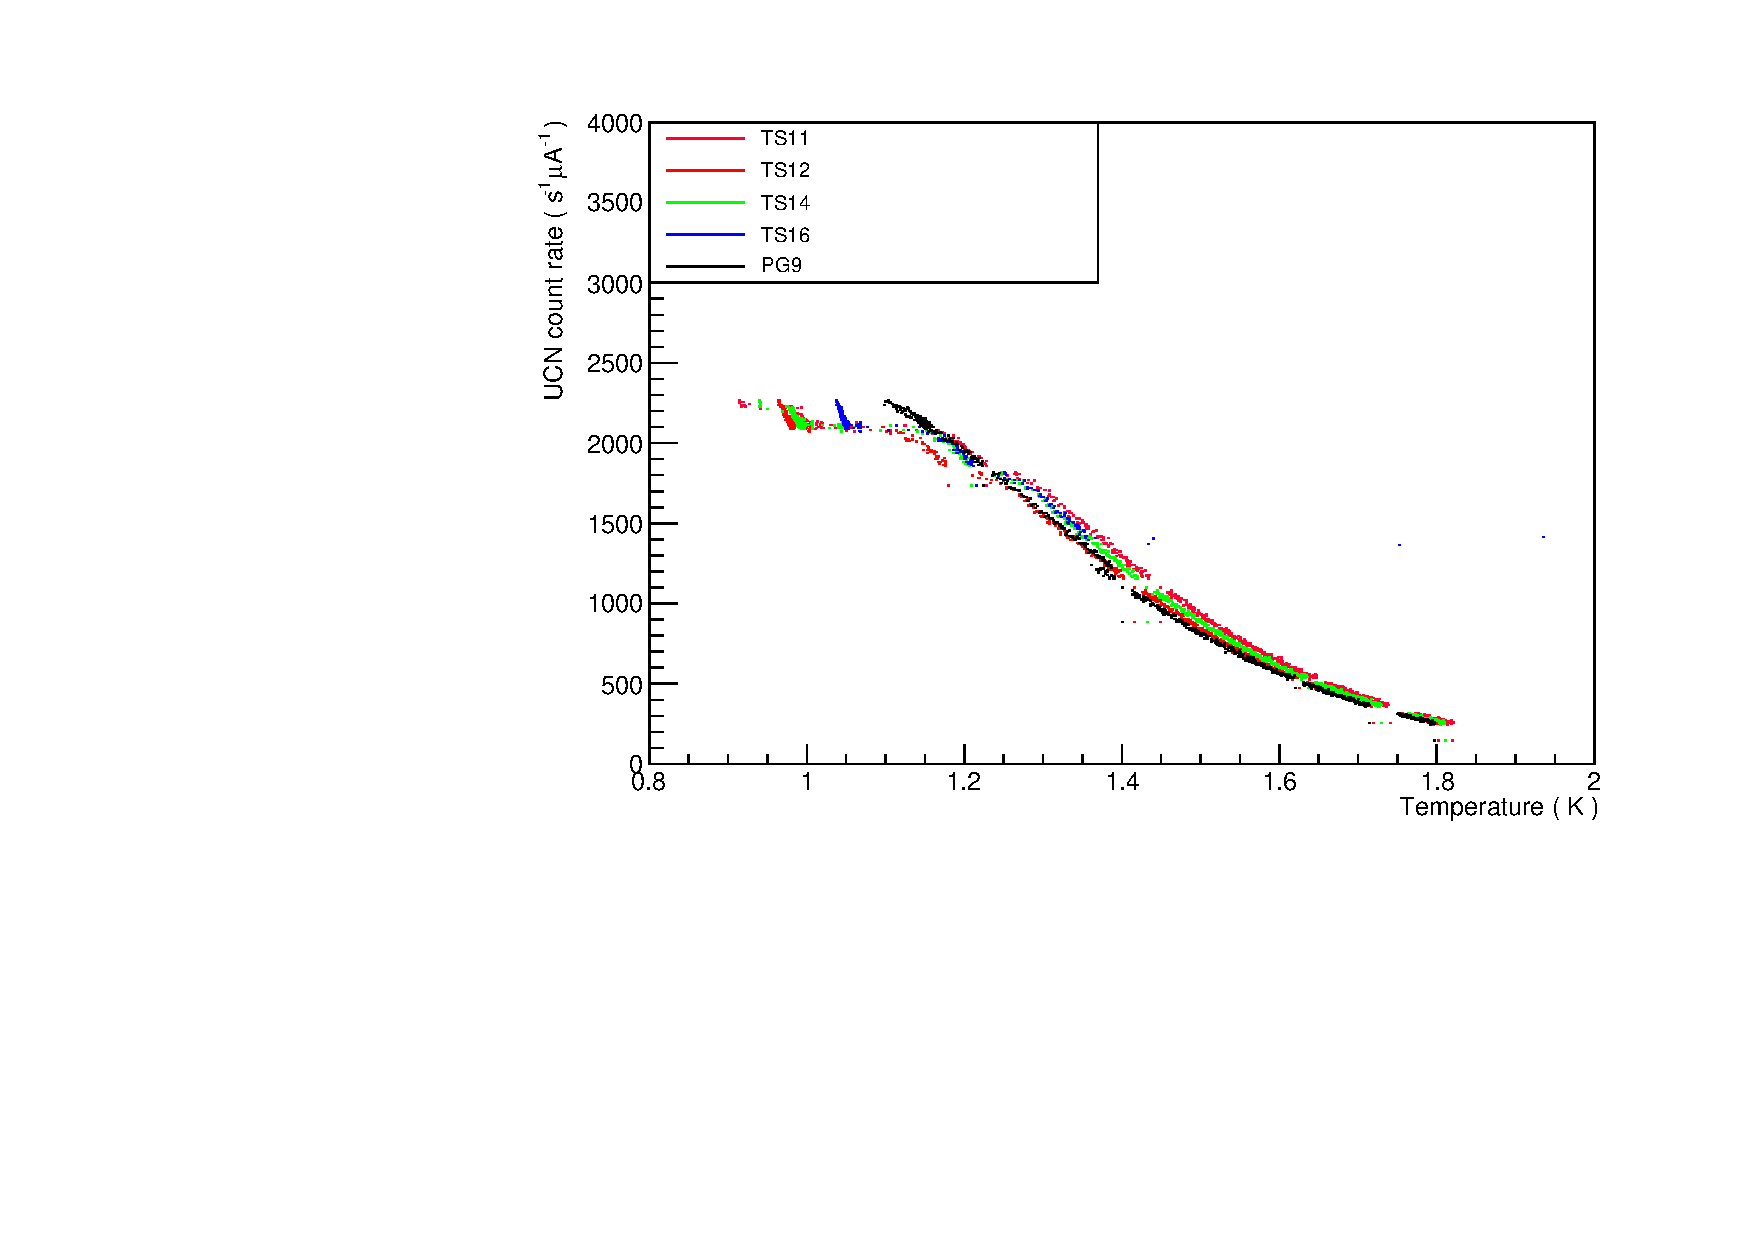
\includegraphics[width=\textwidth,page=1]{../steady_state/li6RateVsTempRun1162.pdf}
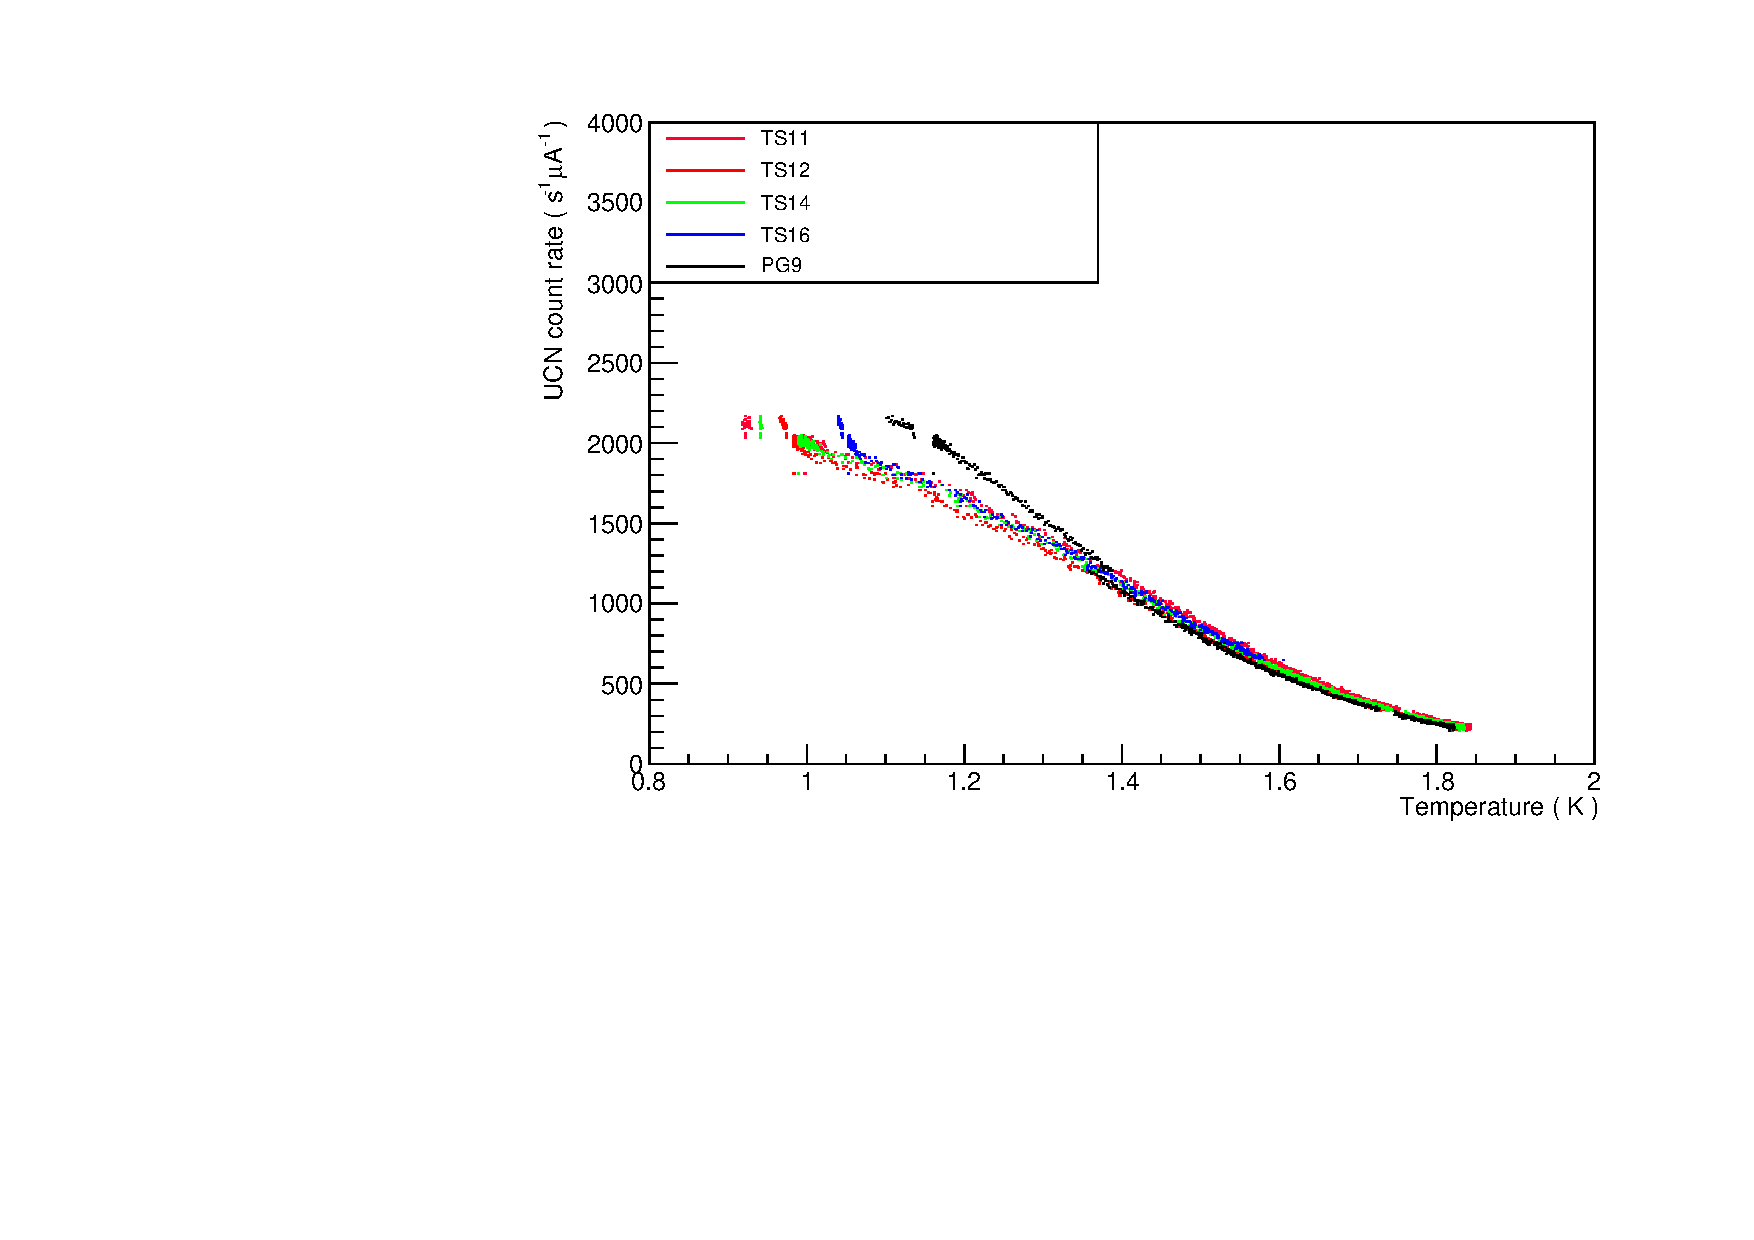
\includegraphics[width=\textwidth,page=1]{../steady_state/li6RateVsTempRun1163.pdf}
\caption{Steady-state UCN count rates in the Li6 detector while warming up (top) and while cooling back down (bottom)}
\label{fig:steadystate}
\end{figure}

In two different cycles, the VAT valve is opened and UCN are continually produced. In one cycle, the source is cooled down during this time, and in the other it is warmed up. The goal of this study is to analyze how the temperature affects the count rates of UCN in the Li-6 and He-3 detectors, and to determine which of the possible temperature measurement devices (TS11, TS12, TS14, TS16 or PG9) gives the most accurate temperature measurement. In the case of PG9, the pressure measurement is converted into a temperature with a temperature-vapour pressure correlation. The count rate is determined by binning the timestamps of Li6 or He3 hits into time bins, and then dividing by the difference between the bins.

To ensure that the data is reliable, several cuts are made. Firstly, every during every period from when the beam current drops below \SI{0.9}{\micro\ampere}, until \SI{60}{\second} after it returns above \SI{0.9}{\micro\ampere}, the data is discarded. Additionally, at any instant in which the VAT valve IV1 is closed, the data is discarded. There are two devices, PG9L and PG9H, which read the vapour pressure. PG9L is a more accurate reading below \SI{2}{\torr}, whereas PG9H is more accurate above \SI{2}{\milli\torr}. Therefore, the reading from PG9L is used when it reads below that threshold, and PG9H is used otherwise. Finally, the experimentally determined background for the Li6 detector is subtracted, and the count rates are normalized to beam current.

Two separate plots of count rate vs temperature are made, for warming up and cooling down, see Fig.~\ref{fig:steadystate}. The count rate is plotted as a function of temperature as measured by each of the different devices. It would appear as though PG9 produces the most accurate measurement.





\section{Background rates}
\label{sec:background}



\section{Reproducibility}


\section{Thermal neutron detector}

\begin{figure}
\centering
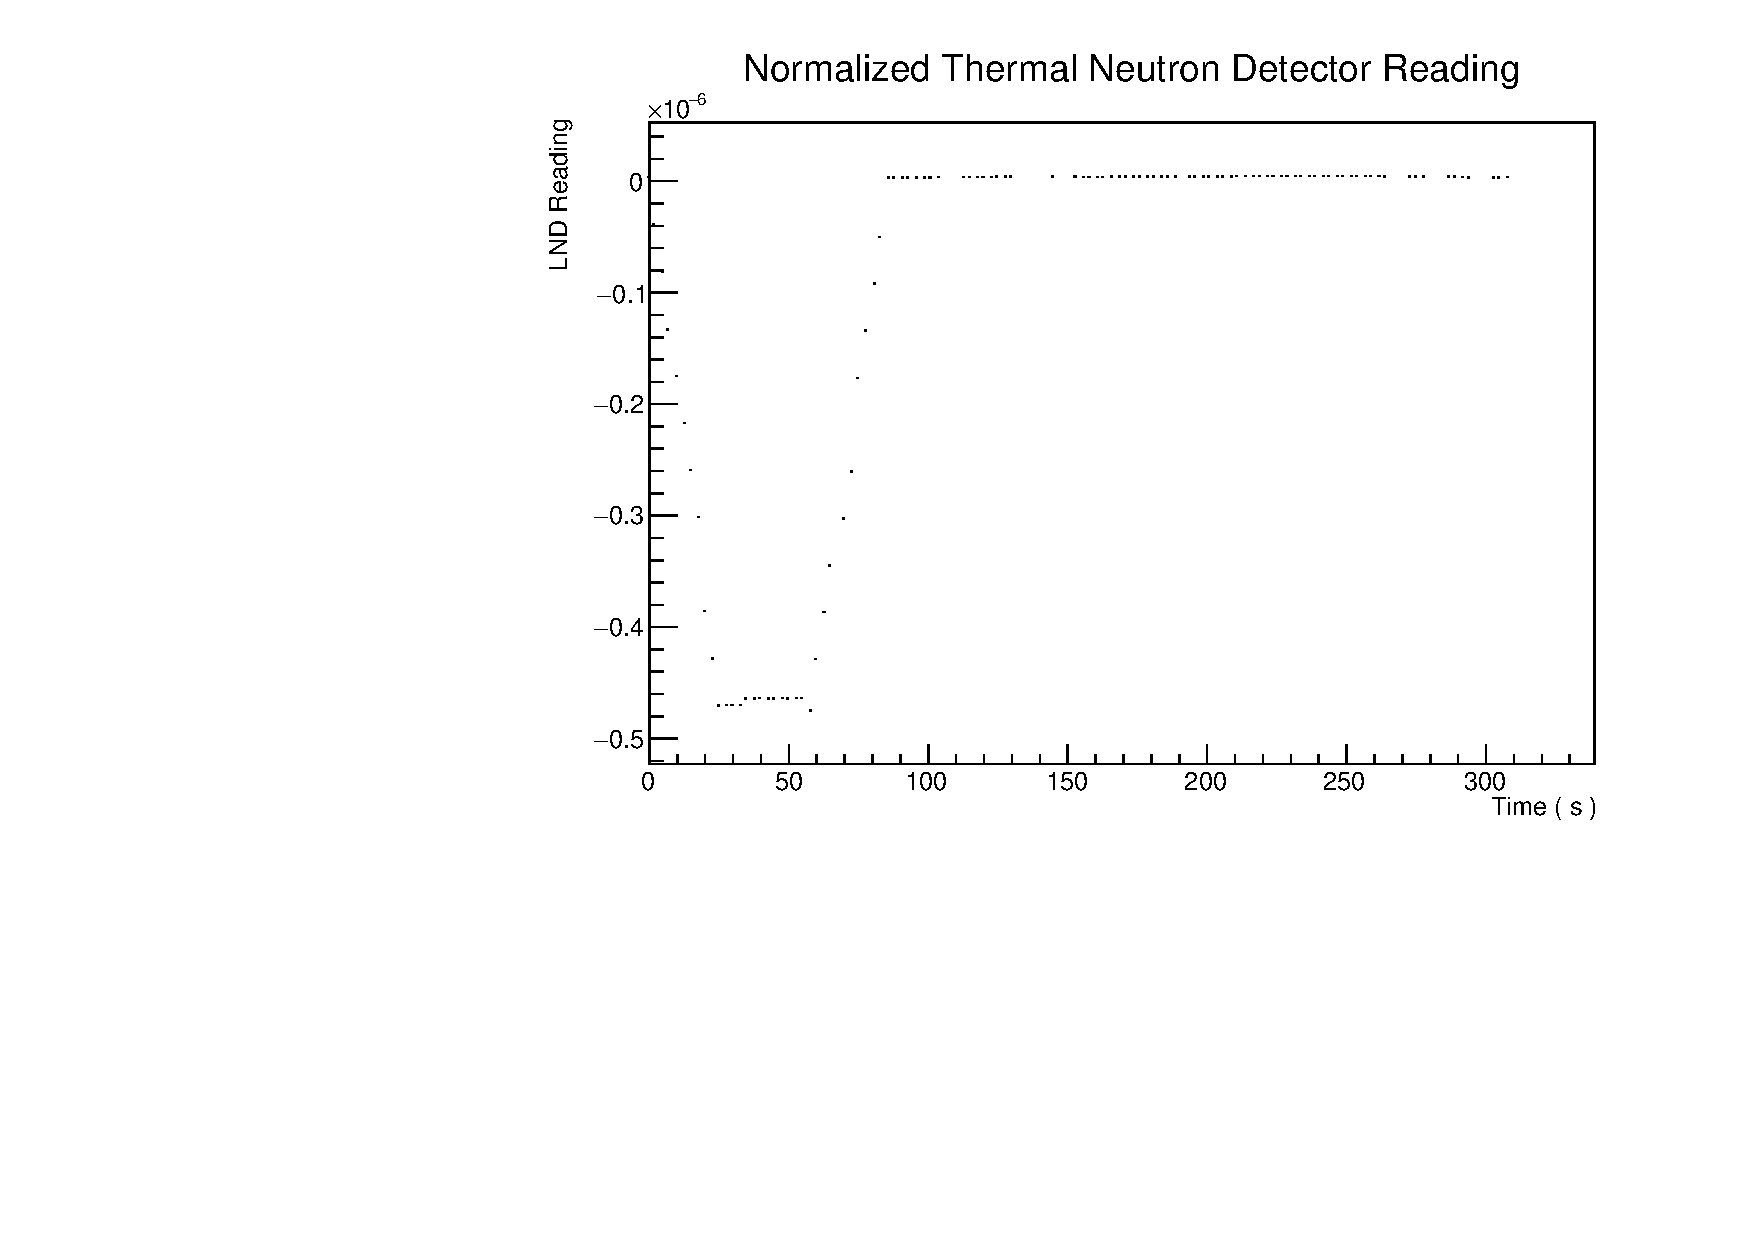
\includegraphics[width=\textwidth,page=1]{../thermal_neutron_detector/lndReadingVsTimeTCN18-042.pdf}
\caption{Thermal neutron detector device reading. Notice the current rising prior to reading a plateau, stabilizing, and then dropping off}
\label{fig:LNDplateau}
\end{figure}

The output on this device is a negative, time-averaged current reading, which will take some time before the reading is accurate. The reading is negative, so the convention adopted for the rest of this section is that when the magntiude of the reading increases (i.e. it becomes more negative), it will be said the the reading has increased. If it becomes more positive, it will be said that the reading has dropped, as it has decreased in magntiude. Some ``buffer'' time is requied until the reading stabilizes. Although it will sometimes stabilize more quickly, this buffer time is set at \SI{30}{\second}. If a cycle is completed before this time is reached (i.e. the beam on duration is less than \SI{30}{\second}), then that cycle is discarded. All of the LND readings between this buffer time and the moment the beam goes off are averaged, and that (negative) plateau is reported as the LND reading. If the cycle ends before the beam goes off, but after \SI{30}{\second}, then all times beyond \SI{30}{\second} are averaged to get the LND reading. An example of the LND reading over time is shown in Fig \ref{fig:LNDplateau}.

\begin{figure}
\centering
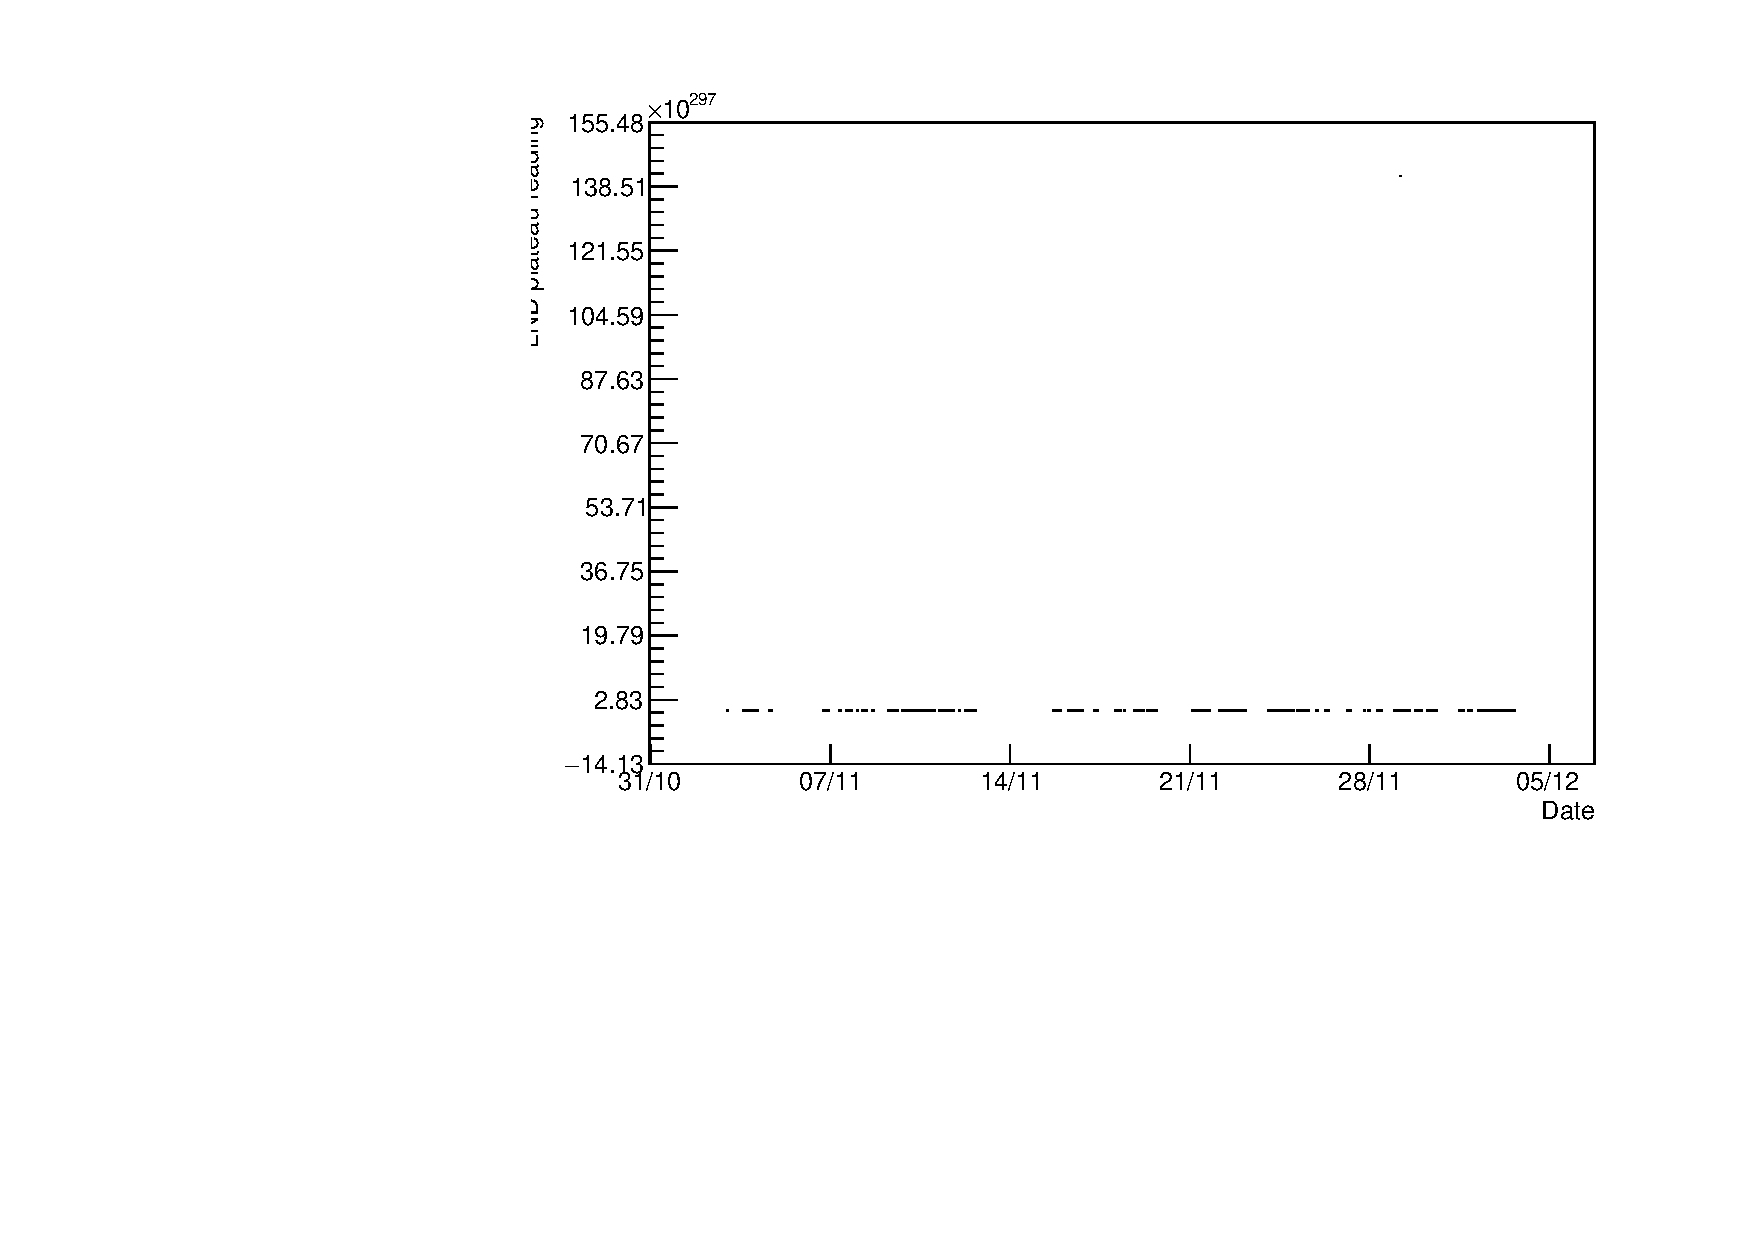
\includegraphics[width=\textwidth,page=1]{../thermal_neutron_detector/lndReadingOverTime.pdf}
\caption{LND plateau reading from valid cycles plotted as function of time. Areas without data points indicate periods of data discarded.}
\label{fig:LNDreadings}
\end{figure}

\begin{figure}
\centering
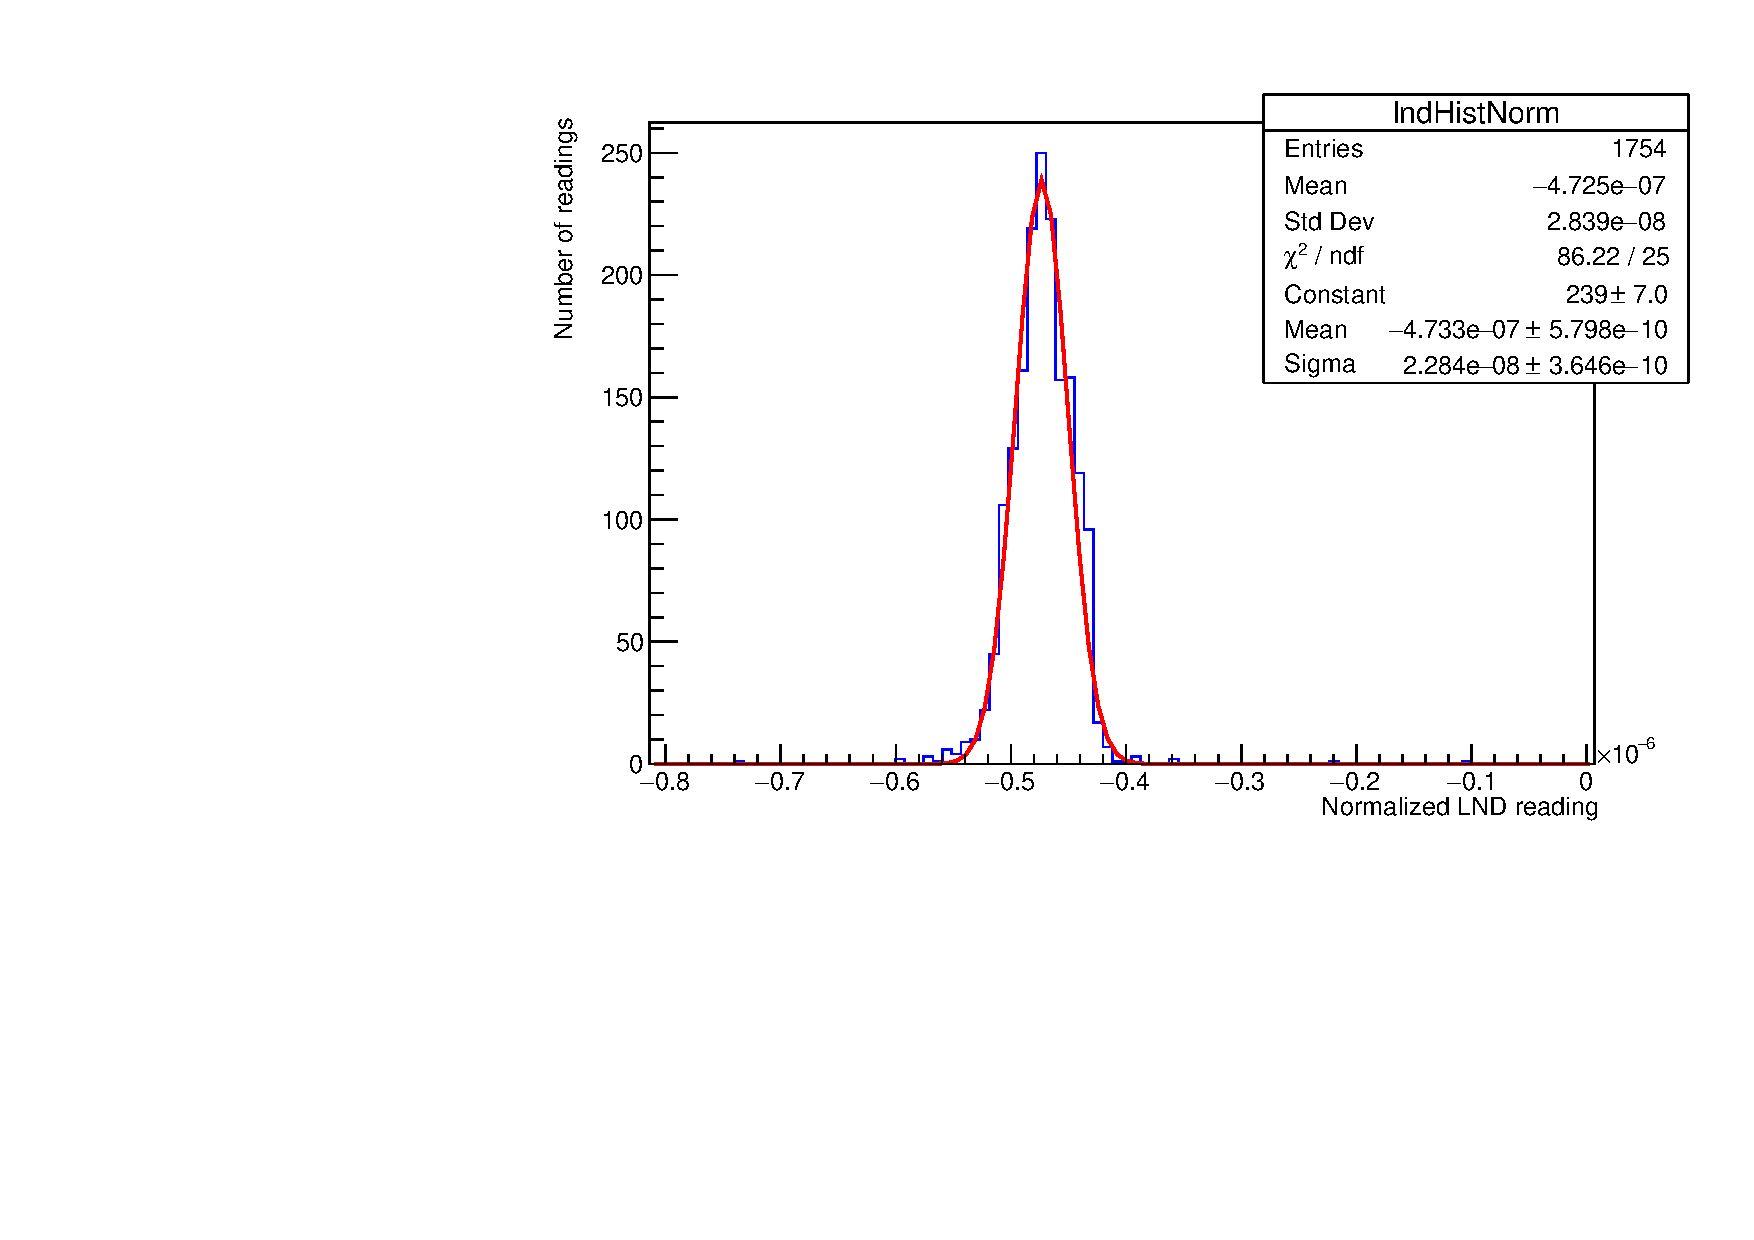
\includegraphics[width=\textwidth,page=1]{../thermal_neutron_detector/lndHist.pdf}
\caption{LND reading normalized by dividing to beam current, with Gaussian fit}
\label{fig:LNDhist}
\end{figure}

Not every cycle has reliable data, however. Cycles in which the beam current drops below \SI{0.1}{\micro\ampere}, or those where the beam fluctuates with a standard deviation of more than \SI{0.02}{\micro\ampere} are discarded. There is also a period from November 16 to November 26 during which the average LND reading drops by $\approx$\SI{0.3}{\micro\ampere}. The cause of this change is uncertain, but it is highly likely that this was due to an issue with the DAQ hardware, and therefore not due to some sudden physical change. Accordingly, all cycles in which the LND plateau is below \SI{0.3}{\micro\ampere} are discarded. Additionally, all those where the reading is above \SI{0.6}{\micro\ampere} are also discarded. There are some cycles in which the device was disabled, and the reading was near zero ($\approx$ \SI{1}{\nano\ampere}). These will be discarded along with those readings associated due to DAQ issues (as in both cases, readings drop below \SI{0.3}{\micro\ampere}). The LND plateau readings of the valid cycles are plotted as a function of time in Fig \ref{fig:LNDreadings}. The readings are then normalized by dividing by beam current, and then are binned in and plotted in Fig \ref{fig:LNDhist}, with a Gaussian fit.

\end{document}
